\section{Décodage}
	\subsection{Principe}
	Un codeur à quadrature de phases se compose d'un stator, avec deux capteurs (généralement des capteurs optiques) et d'un rotor associé à une roue de codage (cf Figure \ref{img:encoderWheel}). Les capteurs aux stators génèrent des signaux de tensions carrés, selon qu'il sont obstrués ou non par les marquages de la roue de codage (on peut voir un exemple Figure \ref{img:schemaQuadrature}).\\
	
	Comme on peut le voir sur la Figure \ref{img:encoderWheel} les marquages de la roue de codage sont légèrement déphasé et ce de telle sortes à ce que les signaux de nos deux capteurs (que l'on appellera signal A et signal B dorénavant). Ainsi, selon le sens de rotation du rotor et de la roue de codage, les signaux A et B auront un déphasage de $\pm 90\deg$. C'est le signe du déphasage qui nous permettra de connaître le sens de rotation.\\
	Il suffit ensuite de compter (ou decompter) les impulsions sur les signaux A et B pour complètement décoder cette information. Le comptage/decomptage nous apporte une information de position, ou plutôt de distance angulaire parcourue par le rotor. On peut aussi facilement en extraire la vitesse ou l'accélération  du rotor, puisqu'il suffit d'utiliser les dérivées en fonction du temps pour obtenir ces informations.\\

	\begin{figure}[h!]
  		\centering
  		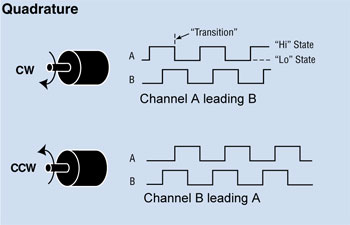
\includegraphics[width=0.5\textwidth]{img/quadrature}
 		\caption{Principe de fonctionnement des codeurs à quadratures de phases}
  		\label{img:schemaQuadrature}
	\end{figure}	

	\begin{figure}[h!]
  		\centering
  		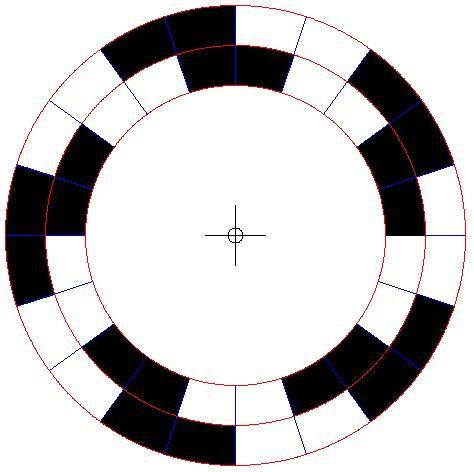
\includegraphics[width=0.3\textwidth]{img/encoderwheel}
 		\caption{Roue de codage}
  		\label{img:encoderWheel}
	\end{figure}	
	
	Après une longue réflexion sur la méthode d'interpretation logique des signaux, nous avons décider de simplement poser la table de vérité de ce mode de fonctionnement.\\
	Comme nous travaillons sur des fronts montants et descendants, nous décidons de travailler sur la valeur de A et de B ainsi que de leurs valeurs au temps précédent (nous supposons un fonctionnement synchrone). Si $A(t)=A$ alors $A^{-1} = A(t-1)$.\\
	
	On retrouve alors 16 cas différents (voir Tableau ci-après).\\
	Pour simplifier l'exercice et améliorer la résolution, nous allons effectuer le comptage/decomptage sur chaque front des deux signaux, ce qui fait 4 fronts par passage devant un marquage de roue (d'où l'augmentation de la résolution par 4).\\
	Cela explique pourquoi dans les cas 1, 2, 4, 7, 8, 11, 13, 14 Count est à 1. Les cas 0, 5, 10 et 15 ne présentent pas de fronts, Count est donc à 0 et les cas 3, 6, 9 et 12 représentent des fronts simultanés sur A et B. Ces cas sont impossible sur un codeurs, mais on choisit d'interdire tout de m\^eme le comptage au cas où, Count est donc à 0.\\
	
	Déjà maintenant nous pouvons définir l'équation logique de Count. Si l'on regarde attentivement la table de vérité quand Count est vrai, il y a toujours un nombre impair de 1 sur les entrées $A,B,A^{-1},B^{-1}$ et inversement. Ce comportement est simplement le comportement de plusieurs ou exclusifs. Ainsi $Count = A \oplus B \oplus A^{-1} \oplus B^{-1}$.\\
	
	Il faut maintenant définir Up et Down.\\
	Il y a d'abord les cas où Count est à 0, il n'est pas nécessaire de conna\^itre le sens de comptage à ce stage, puisqu'il n'y a pas de comptage à effectuer. On fixe alors leur état à l'état indifférent pour pouvoir ensuite faire quelques simplifications.\\
	On va ensuite regarder chaque cas et analyser l'état, par exemple un front montant sur B avec A encore au niveau bas indique que le signal B précède A (un front montant sur A devrait arrivé avec un déphasage de $90\deg$). En revanche, un front descendant sur B avec A déjà en niveau bas indique que cette fois-ci le signal A précède B.\\
	En suivant ce raisonnement on obtient la table de vérité suivante : \\
	
	\begin{tabular}{|l|||c|c|c|c|||c|c||c|}
	  \hline
	  Cas & $A$ & $B$ & $A^{-1}$ & $B^{-1}$ & Up & Down & Count \\
	  \hline
	  \hline
	  0 &0&0&0&0&X&X&0 \\
	  \hline
	  1 &0&0&0&1&0&1&1 \\
	  \hline
	  2 &0&0&1&0&1&0&1 \\
	  \hline
	  3 &0&0&1&1&X&X&0 \\
	  \hline
	  4 &0&1&0&0&1&0&1 \\
	  \hline
	  5 &0&1&0&1&X&X&0 \\
	  \hline
	  6 &0&1&1&0&X&X&0 \\
	  \hline
	  7 &0&1&1&1&0&1&1 \\
	  \hline
	  8 &1&0&0&0&0&1&1 \\
	  \hline
	  9 &1&0&0&1&X&X&0 \\
	  \hline
	  10 &1&0&1&0&X&X&0 \\
	  \hline
	  11 &1&0&1&1&1&0&1 \\
	  \hline
	  12 &1&1&0&0&X&X&0 \\
	  \hline
	  13 &1&1&0&1&1&0&1 \\
	  \hline
	  14 &1&1&1&0&0&1&1 \\
	  \hline
	  15 &1&1&1&1&X&X&0 \\
	  \hline
	\end{tabular}~\\
	
	En posant $C = A^{-1}$ et $D = B^{-1}$, on peut alors représenter cette table de vérité pour Down avec le tableau de Karnaugh de la Figure \ref{img:Karnaugh}.\\
		
	\begin{figure}[h!]
  		\centering
  		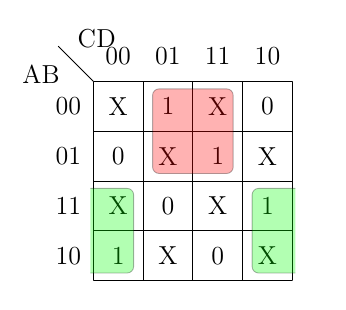
\includegraphics[width=0.3\textwidth]{img/Karnaugh}
 		\caption{Tableau de Karnaugh}
  		\label{img:Karnaugh}
	\end{figure}	

On obtient alors, après simplifications, l'équation logique suivante : $Down = A.\overline{B^{-1}} + \overline{A}.B^{-1} = A \oplus B^{-1}$.\\

Il faut ensuite implémenter la solution VHDL, et cela devient très appréciable puisque le code du process de décodage tiens dans une vingtaine de ligne. Ça n'a rien de comparable aux autres solutions testées (qui étaient encore trop calquées sur le schéma de réflexion sur micro-contrôleur).\\

\newpage
Voici le process synchrone complet : \\
\begin{lstlisting}
process (clk) begin
  if (clk'event and clk='1') then
    up <= A XOR B_delayed;
    enable <= A XOR B XOR A_delayed XOR B_delayed;
    A_delayed <= A;
    B_delayed <= B;

    if (reset='0') then
        if (enable='1') then
            if (up='1') then
               count_register <= count_register+1;
            else
                count_register <= count_register-1;
            end if;
        end if;
    else
        count_register <= (others =>'0');
    end if;
  end if;
end process;
\end{lstlisting}

	\newpage
		% Adaptation de tensions		
	\subsection{Adaptation de tension}
	Le FPGA et la carte de développement cible de notre projet ont la particularité de travailler avec des tensions de 3,3V.\\
	Nos encodeurs eux sont alimentés en 5V, et un branchement direct risquerait d'endommager le FPGA.\\
	
	Fort heureusement pour deux de nos encodeurs, leurs sorties est dite à collecteur ouvert. Cela signifie que leur état est soit à haute impédance, soit à GND.\\
	C'est un gros avantage pour nous, puisqu'il suffit de travailler avec une résistance de tirage placée sur du 3,3V pour que la sortie du codeur passe de (Haute Impédance/GND à 3,3V/GND). Qui plus est, les FPGA propose de configurer directement ses entrées (par le biais du fichier de contrainte) en mode pull-up.\\
	Pour ces deux encodeurs, on a donc une pleine compatibilité.\\
	
	Les encodeurs placés à l'arrière de nos moteurs électriques n'avait pas cet atout là. Il nous a donc fallut adapter leur tension.\\
	Initialement nous avons pensé à utiliser des circuits intermédiaires tolérant un signal de 5V et travaillant en 3,3V. \\
	Pour des raisons de simplicités et de co\^uts, nous nous sommes contentés de l'utilisation de ponts diviseur de tensions pour convertir les signaux et les utiliser sur le FPGA.\\
	Cela fonctionne correctement.\\
	
	Cette adaptation de tension peut parra\^itre anodine mais il est important de penser à ce genre de choses puisque la carte n'est absolument pas protégée contre ça et une mauvaise utilisation ou configuration aurait endommagé la carte.\\
	
		% Problème de rebonds
	\subsection{Problème de rebonds}
	Assez rapidement nous avons rencontré un problème qui n'était pas présent en simulation.\\
	Sur la simulation le comptage et le décomptage s'effectuait sans aucun problème et était fidèle.\\
	
	En pratique, là où un tour complet du rotor devait amener un niveau de compteur de $4\times 1024 = 4096$, on obtenait plut\^ot des valeurs de 4300, 4600 ticks/tours. Ce n'était absolument pas satisfaisant et nous n'en comprenions pas la cause.\\
	
	A force de recherches et avec le secours d'un analyseur logique, nous avons pu repérer l'origine du problème.\\
	On peut voir en Figure \ref{img:zoomBounce} et \ref{img:Bounce} un phénomène de rebonds.\\ 
	Le signal analogique correspond au signal B et D9 est son interprétation logique par le FPGA. On voit que lors de l'établissement du signal, il y a des erreurs d'interprétations de la part du FPGA qui parfois confond les deux niveaux logiques.\\
	Lorsque l'on zoom, on voit clairement plusieurs rebonds et ils ont une conséquence sur le signal de comptage (D14). On voit par exemple sur notre zoom que pour ce front montant, l'application à compter au moins deux fois.\\
	
	\begin{figure}[h!]
  		\centering
  		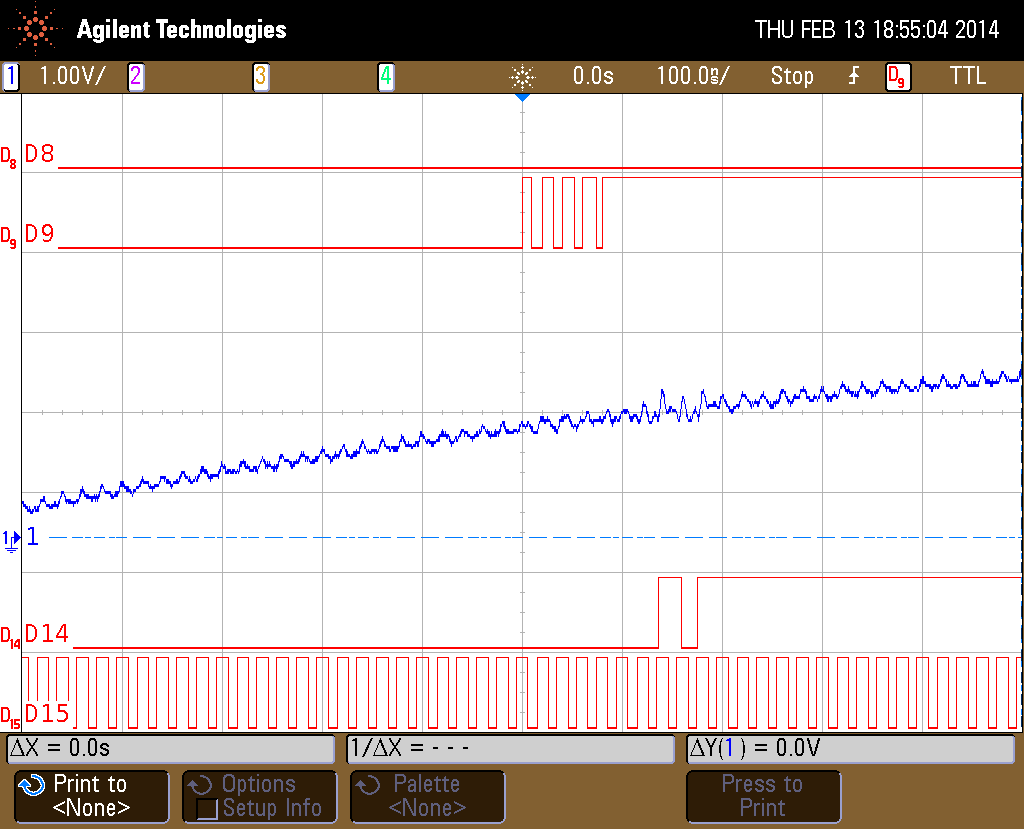
\includegraphics[width=0.7\textwidth]{img/scope_0}
 		\caption{Zoom sur les rebonds}
  		\label{img:zoomBounce}
	\end{figure}	
	\begin{figure}[h!]
  		\centering
  		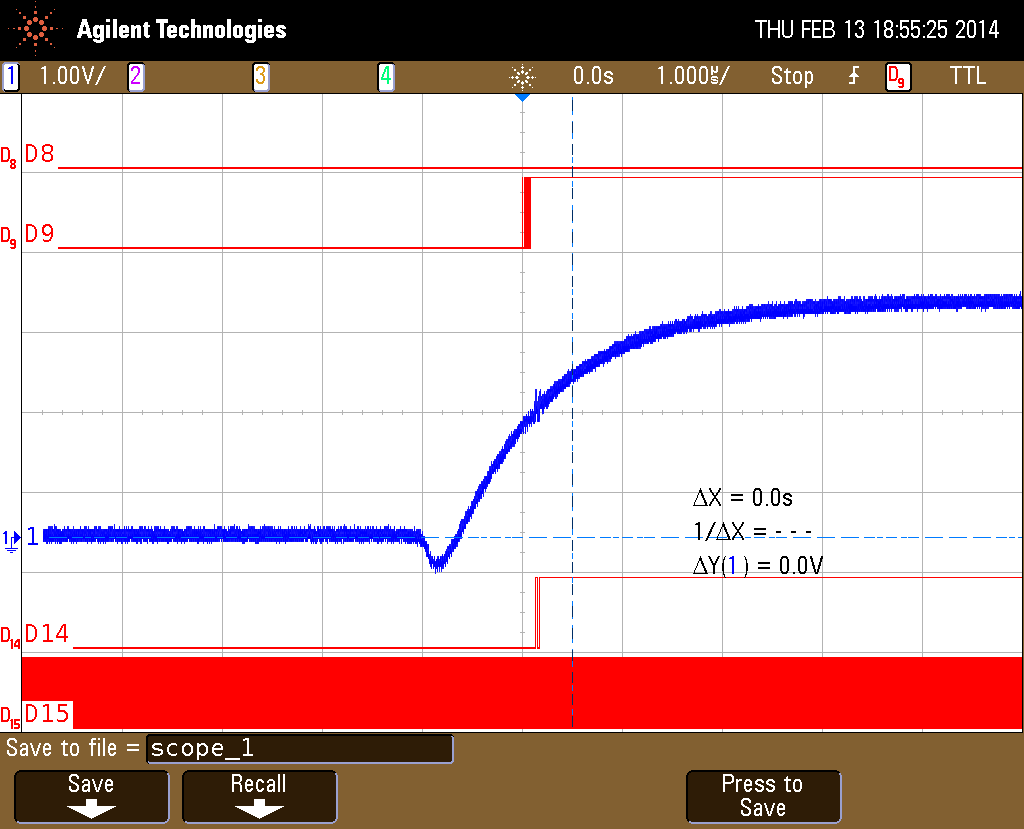
\includegraphics[width=0.7\textwidth]{img/scope_1}
 		\caption{Problème de rebonds à l'établissement du signal}
  		\label{img:Bounce}
	\end{figure}	
	
	Pour répondre au problème nous avons tenter d'utiliser un filtrage, mais cela a échoué, ce n'était pas vraiment la bonne solution.\\
	Nous avons aussi pensé à un trigger de schmidt qui assurerait des niveaux fiables et avec un temps d'établissement très court. Cette solution n'a pas été testé puisque nous avons choisis d'utiliser encore une fois les ressources du FGPA en utilisant des modules anti-rebonds en VHDL développé par Mickael Coronado, Ingénieur Electronique Analogique / Numérique (Spécialiste FPGA) et Dirigeant (entreprise Inodesign) et aussi à l'origine de ce projet.\\
	
	Cette solution permet de s'assurer que les signaux sont valides en vérifiant qu'ils restent invariants pendant plusieurs fronts d'horloges. Elle s'avère très efficace.\\